%"The PDF file may contain up to 25 pages of reference material, single-sided, letter or A4 size, with text and illustrations readable by a person with correctable eyesight without magnification from a distance of 1/2 meter."
\documentclass[10pt,landscape,twocolumn,a4paper,notitlepage]{article}
\usepackage{hyperref}
\usepackage[english, activeacute]{babel}
\usepackage[utf8]{inputenc}
\usepackage{fancyhdr}
\usepackage{lastpage}
\usepackage{listings}
\usepackage{amssymb}
\usepackage[usenames,dvipsnames]{color}
\usepackage{graphicx}
\usepackage{wrapfig}
\usepackage{amsmath}
\usepackage{makeidx}
\usepackage[document]{ragged2e}
\usepackage[usestackEOL]{stackengine}[2013-10-15]
\def\x{\hspace{3ex}}    %BETWEEN TWO 1-DIGIT NUMBERS
\def\y{\hspace{2.45ex}}  %BETWEEN 1 AND 2 DIGIT NUMBERS
\def\z{\hspace{1.9ex}}    %BETWEEN TWO 2-DIGIT NUMBERS
\stackMath

%%% Margenes
\setlength{\columnsep}{0.25in}    % default=10pt
\setlength{\columnseprule}{0.5pt}    % default=0pt (no line)

\addtolength{\textheight}{2.35in}
\addtolength{\topmargin}{-0.9in}     % ~ -0.5 del incremento anterior

\addtolength{\textwidth}{1.1in}
\addtolength{\oddsidemargin}{-0.55in} % -0.5 del incremento anterior

\setlength{\headsep}{0.08in}
\setlength{\parskip}{0in}
\setlength{\headheight}{15pt}
\setlength{\parindent}{0mm}

%%% Encabezado y pie de pagina
\pagestyle{fancy}
\fancyhead[LO]{\textbf{\title}}
\fancyhead[C]{\leftmark\ -\ \rightmark}
\fancyhead[RO]{Page \thepage\ of \pageref{LastPage}}
\renewcommand{\headrulewidth}{0.4pt}
\fancyfoot{}
\definecolor{darkblue}{rgb}{0,0,0.4}
%%% Configuracion de Listings
\lstloadlanguages{C++}
\lstnewenvironment{code}
	{%\lstset{	numbers=none, frame=lines, basicstyle=\small\ttfamily, }%
	 \csname lst@SetFirstLabel\endcsname}
	{\csname lst@SaveFirstLabel\endcsname}
\lstset{% general command to set parameter(s)
	language=C++, basicstyle=\small\ttfamily, keywordstyle=\slshape,
	emph=[1]{tipo,usa}, emphstyle={[1]\sffamily\bfseries},
	morekeywords={tint,forn,forsn,fore},
	basewidth={0.47em,0.40em},
	columns=fixed, fontadjust, resetmargins, xrightmargin=5pt, xleftmargin=15pt,
	flexiblecolumns=false, tabsize=2, breaklines,	breakatwhitespace=false, extendedchars=true,
	numbers=left, numberstyle=\tiny, stepnumber=1, numbersep=9pt,
	frame=l, framesep=3pt,
    basicstyle=\ttfamily,
    keywordstyle=\color{darkblue}\ttfamily,
    stringstyle=\color{magenta}\ttfamily,
    commentstyle=\color{RedOrange}\ttfamily,
    morecomment=[l][\color{OliveGreen}]{\#}
}

\lstdefinestyle{C++}{
	language=C++, basicstyle=\small\ttfamily, keywordstyle=\slshape,
	emph=[1]{tipo,usa,tipo2}, emphstyle={[1]\sffamily\bfseries},
	morekeywords={tint,forn,forsn,fore},
	basewidth={0.47em,0.40em},
	columns=fixed, fontadjust, resetmargins, xrightmargin=5pt, xleftmargin=15pt,
	flexiblecolumns=false, tabsize=2, breaklines,	breakatwhitespace=false, extendedchars=true,
	numbers=left, numberstyle=\tiny, stepnumber=1, numbersep=9pt,
	frame=l, framesep=3pt,
    basicstyle=\ttfamily,
    keywordstyle=\color{darkblue}\ttfamily,
    stringstyle=\color{magenta}\ttfamily,
    commentstyle=\color{RedOrange}\ttfamily,
    morecomment=[l][\color{OliveGreen}]{\#}
}

%%% Macros
\def\nbtitle#1{\begin{Large}\begin{center}\textbf{#1}\end{center}\end{Large}}
\def\nbsection#1{\section{#1}}
\def\nbsubsection#1{\subsection{#1}}
\def\nbcoment#1{\begin{small}\textbf{#1}\end{small}}
\newcommand{\comb}[2]{\left( \begin{array}{c} #1 \\ #2 \end{array}\right)}
\def\complexity#1{\texorpdfstring{$\mathcal{O}(#1)$}{O(#1)}}
 \newcommand\cppfile[2][]{
\lstinputlisting[style=C++,linerange={#1}]{#2}
}

\begin{document}
\def\title{Universidad Autonoma de Ciudad Juarez - First to Penalty}
.\\[0.2cm]
\centering{\LARGE\textbf{First to Penalty}} \\[0.5cm]
\centering{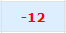
\includegraphics[width=5.5cm]{penalty.png}}
\tableofcontents\newpage

\section{Template}
\cppfile{template.cpp}

\section{Data structures}
\subsection{struct}
\cppfile{data_structures/costocarretera.cpp}
\subsection{segTree}
\cppfile{data_structures/segmentTreeGlobal.cpp}


\section{Graphs}
\subsection{bfs}
\cppfile{graphs/bfs.cpp}
\subsection{dfs}
\cppfile{graphs/dfs.cpp}

\section{Math}
\subsection{Coeficientes binomiales. (Combinaciones n en k)}
\begin{justify}
Una combinación es una forma de elegir $k$ elementos de un grupo de tamaño $n$, sin importar el orden en que los eliges.
\end{justify}
\begin{equation*}
    \binom{n}{k} = \frac{n!}{k!(n-k)!}
\end{equation*}
\begin{equation*}
    (a+b)^{n} = \sum_{k = 0}^{n} \binom{n}{k}a^{n-k}b^{k}
\end{equation*}
\begin{equation*}
    \binom{n}{k} = \binom{n}{n-k}
\end{equation*}
\begin{equation*}
    \binom{n}{k} = \binom{n-1}{k} + \binom{n-1}{k-1}
\end{equation*}
\begin{equation*}
    k\binom{n}{k} = n\binom{n-1}{k-1}
\end{equation*}
\begin{equation*}
    \sum_{k = 0}^{n}\binom{n}{k} = 2^{n}
\end{equation*}
\begin{equation*}
    \sum_{k = 0}^{n} (-1)^{k}\binom{n}{k} = 0
\end{equation*}
\begin{equation*}
    \binom{n+m}{t} = \sum_{k = 0}^{t}\binom{n}{k}\binom{m}{t-k}
\end{equation*}
\begin{equation*}
    \sum_{j = k}^{n} \binom{j}{k} = \binom{n+1}{k+1}
\end{equation*}

\Longstack[l]{
n=0\\
n=1\\
n=2\\
n=3\\
n=4\\
n=5\\
n=6\qquad\ \\
}
\Longstack{
1\\
1\x 1\\
1\x 2\x 1\\
1\x 3\x 3\x 1\\
1\x 4\x 6\x 4\x 1\\
1\x 5\y 10\z 10\y 5\x 1\\
1\x 6\y 15\z 20\z 15\y 6\x 1\\
\overline{0\x 1\x 2\x 3\x 4\x 5\x 6}
}
\Longstack[l]{
n=0\\
n=1\\
n=2\\
n=3\\
n=4\\
n=5\\
n=6\qquad\ \\
}
\Longstack[l]{
1\\
1\x 1\\
1\x 2\x 1\\
1\x 3\x 3\x 1\\
1\x 4\x 6\x 4\x 1\\
1\x 5\y 10\z 10\y 5\x 1\\
1\x 6\y 15\z 20\z 15\y 6\x 1\\
\overline{0\x 1\x 2\x 3\x 4\x 5\x 6}
}

\subsection{Numeros catalanes}
\begin{justify}
Los números de Catalan son una secuencia de números enteros que aparecen en varios problemas combinatorios y estructurales en matemáticas. Se utilizan para contar estructuras específicas que siguen reglas particulares, como el número de maneras de emparejar paréntesis correctamente, las maneras de dividir un polígono convexo en triángulos, o las maneras de construir árboles binarios completos.
\\
Los números de Catalan también se aplican en la cuenta de caminos específicos, aunque no para cualquier tipo de camino. En particular, se usan para contar caminos restringidos en una cuadrícula.
\\
Un ejemplo clásico es el conteo de caminos que van desde el punto $(0,0)$ hasta el punto $(n,n)$ en una cuadrícula, avanzando solo hacia la derecha o hacia abajo, pero con la condición de que el camino nunca debe cruzar la diagonal principal (es decir, que en todo momento debe estar por encima o sobre la línea $y = x$. En este contexto, el número de caminos que cumplen esta restricción para una cuadrícula de tamaño $n$ es el n-ésimo número de Catalan.
\end{justify}
\begin{equation*}
    C_{n+1} = \sum_{i=0}^nC_iC_{n-i}
\end{equation*}
%Una fórmula cerrada para los números de Catalán es:
\begin{equation*}
    C_n = \frac{1}{n+1}\binom{2n}{n} = \binom{2n}{n} - \binom{2n}{n+1}
\end{equation*}

\begin{equation*}
    C_n = \frac{2(2n-1)}{n+1} C_{n-1}
\end{equation*}

\begin{equation*}
    C_n \approx \frac{4^n}{n^{3/2}\sqrt{\pi}}
\end{equation*}

\subsection{Separadores o barras y estrellas}
\begin{justify}
En combinatoria, el método de separadores (o barras y estrellas) es una técnica para contar formas de dividir $n$ objetos idénticos en $k$ grupos.
\\
Imagina que tienes $n$ caramelos idénticos y quieres repartirlos entre $k$ niños. Para resolver esto, colocas $k-1$ separadores entre los caramelos, dividiendo el total en $k$ partes. Cada parte representa la cantidad de caramelos que cada niño recibe, y puede ser cero.
\\
El numero de formas de hacer esto es $\binom{n+k-1}{k-1}$ ya que estamos eligiendo posiciones para los separadores entre los $n+k-1$ espacios disponibles.
\end{justify}
\begin{equation*}
    \left(\binom{n}{k}\right) = \binom{n-1}{k-1} = \binom{n+k-1}{k-1}
\end{equation*}


\subsection{Permutaciones}
\begin{justify}
Una permutación es una forma de elegir y organizar $k$ elementos de un grupo de tamaño $n$, donde el orden sí importa. (i.e. 1,2,3 es diferente a 3,1,2)
\end{justify}
\begin{equation*}
    P(n,k) = \frac{n!}{(n-k)!}
\end{equation*}
\textbf{Permutaciones objetos repetidos}
\begin{justify}
Si existen elementos iguales entre los que hay que elegir (i.e. CARTA tiene dos 'A'), definamos la cantidad que ocurre el i-esimo elemento como $am_{i}$ (as in amount)-
\end{justify}
\begin{equation*}
    P(n,k) = \frac{P(n,k)}{e_{1}!e_{2}!...} = \frac{n!}{(n-k)!e_{1}!e_{2}!...}
\end{equation*}
\subsection{Derangement} 
\begin{justify}
Un Derangement es una permutación que no deja ningún elemento en su lugar original.
\end{justify}
      \begin{equation*}
        Derangement(n)=
        \begin{cases}
			0 & \text{si $n = 1$}.\\
			1 & \text{si $n = 2$}.\\
			(n - 1)( Derangement(n - 1) + Derangement(n - 2) ) & \text{otherwise}.\\
		\end{cases}
      \end{equation*}

      \begin{equation*}
        Derangement(n) = n! \sum_{k = 0}^n \frac{(-1)^k}{k!}
      \end{equation*}
\subsection{Numeros de Fibonacci}
\begin{equation*}
  F_{n} = F_{n-1}+F_{n-2} 
\end{equation*}
\begin{equation*}
  F_{2n+1} = F_{n}^2 + F_{n+1}^2
\end{equation*}
\begin{equation*}
    F_{2n} = F_{n+1}^2 - F_{n-1}^2
\end{equation*}
\begin{equation*}
    \sum_{i=1}^n F_i = F_{n+2}-1
\end{equation*}
\begin{equation*}
    F_{n+i}F_{n+j} - F_nF_{n+i+j} = (-1)^n F_iF_j
\end{equation*}
\subsection{Cantidad de divisores}
\begin{justify}
Para encontrar la cantidad de divisores de un número, se usa su \textit{factorización prima}. Supongamos que un número $ N$ se factoriza como:
\end{justify}
\begin{equation*}
    N = p_1^{e_1} \times p_2^{e_2} \times \cdots \times p_k^{e_k}
\end{equation*}
\begin{justify}
donde ($p_1, p_2, \dots, p_k$) son los factores primos distintos de $N$, y ($e_1, e_2, \dots, e_k$) son sus respectivos exponentes.
\\
Para obtener la cantidad total de divisores de $N$, se toma cada exponente, se le suma uno, y luego se multiplican todos estos valores:
\end{justify}
\begin{equation*}
    \text{Cantidad de divisores} = (e_1 + 1) \times (e_2 + 1) \times \cdots \times (e_k + 1)
\end{equation*}
\begin{justify}
Para fines de programacion competitiva, considera que $N$ tiene aproximadamente $\sqrt[3]{N}$ divisores.
\end{justify}
\subsection{Respuesta modulo m}
\begin{justify}
En programacion competitiva, es comun encontrar problemas cuya respuesta pueda exceder el limite de long long int de C++ ($10^{18}$), por lo que para mantener la respuesta en un rango aceptable se pide calcularla modulo $m$.
\\
Para calcular una respuesta modulo $m$, es necesario construir el codigo tomando en cuenta las siguientes propiedades.
\end{justify}
\begin{equation*}
    (a+b)\%m = (a\%m + b\%m)\%m
\end{equation*}

\begin{equation*}
    (a-b)\%m = (a\%m - b\%m + m)\%m
\end{equation*}
\begin{equation*}
    (a*b)\%m = (a\%m * b\%m)\%m
\end{equation*}
\begin{justify}
En el caso de divisiones es necesario calcular el inverso modular del divisor, expresado por $b^{-1}$, esto esta codificado en modinverse.
\end{justify}
\begin{equation*}
    (a/b)\%m = (a\%m * (b^{-1})\%m)\%m
\end{equation*}

\subsection{bits}
\cppfile{math/bits.cpp}
\subsection{gcd\_lcm}
\cppfile{math/gcd_lcm.cpp}
\subsection{min\_sum\_sq}
\cppfile{math/min_sum_sq.cpp}
\subsection{mod}
\cppfile{math/mod.cpp}
\subsection{perm\_comb}
\cppfile{math/perm_comb.cpp}

\section{Geometry}


\section{Strings}
\subsection{Common}
\cppfile{strings/common.cpp}
\subsection{KMP}
\cppfile{strings/kmt.cpp}


\section{Flow}


\section{Miscellaneous}
\subsection{Backtracking}
\cppfile{misc/backtracking.cpp}
\subsection{Binary Search}
\cppfile{misc/binarysearch.cpp}
\subsection{Dijsktra}
\cppfile{misc/dijsktra.cpp}
\subsection{knapsack}
\cppfile{misc/knapsack.cpp}
\subsection{laberinto}
\cppfile{misc/laberinto.cpp}
\subsection{lcs}
\cppfile{misc/lcs.cpp}
\subsection{most\_data\_structures}
\cppfile{misc/most_data_structures.cpp}
\subsection{num\_prime\_factors}
\cppfile{misc/num_prime_factors.cpp}
\subsection{primes\_in\_range}
\cppfile{misc/primes_in_range.cpp}
\subsection{weird\_input}
\cppfile{misc/weird_input.cpp}

%\subsection{Bit Manipulation}
%\cppfile{Miscellaneous/bitManip.cpp}
%\cppfile{Miscellaneous/moreBitManin.cpp}

\section{Testing}



\end{document}

